\documentclass[12pt]{article}
\usepackage[english]{babel}
\usepackage[utf8]{inputenc}

%% Pointer to 'default' preamble, other reusable files
% pacakages and definitions

\usepackage{geometry}
\geometry{
	letterpaper, 
	portrait, 
	top=.75in,
	left=.8in,
	right=.75in,
	bottom=.5in		} 	% Page Margins
	
%% additional packages for nice things
\usepackage{amsmath} 	% for most math
\usepackage{commath} 	% for abs
\usepackage{lastpage}	% for page count
\usepackage{amssymb} 	% for therefore
\usepackage{graphicx} 	% for image handling
\usepackage{wrapfig} 	% wrap figures
\usepackage[none]{hyphenat} % for no hyphenations
\usepackage{array} 		% for >{} column characterisctis
\usepackage{physics} 	% for easier derivative \dv....
\usepackage{tikz} 		% for graphic@!
\usepackage{circuitikz} % for circuits!
\usetikzlibrary{arrows.meta} % for loads
\usepackage[thicklines]{cancel}	% for cancels
\usepackage{xcolor}		% for color cancels
\usepackage[per-mode=fraction]{siunitx} % for si units and num
\sisetup{group-separator = {,}, group-minimum-digits = 3} % additional si unit table functionality

\usepackage{fancyhdr} 	% for header
\usepackage{comment}	% for ability to comment out large sections
\usepackage{multicol}	% for multiple columns using multicols
\usepackage[framed,numbered]{matlab-prettifier} % matlab sytle listing
\usepackage{marvosym} 	% for boltsymbol lightning
\usepackage{pdflscape} 	% for various landscape pages in portrait docs.
%\usepackage{float}
\usepackage{fancyvrb}	% for Verbatim (a tab respecting verbatim)
\usepackage{enumitem}	% for [resume] functionality of enumerate
\usepackage{spreadtab} 	% for using formulas in tables}
\usepackage{numprint}	% for number format in spread tab
\usepackage{subcaption} % for subfigures with captions
\usepackage[normalem]{ulem} % for strike through sout

% for row colors in tables....
\usepackage{color, colortbl}
\definecolor{G1}{gray}{0.9}
\definecolor{G2}{rgb}{1,0.88,1}%{gray}{0.6}
\definecolor{G3}{rgb}{0.88,1,1}

% For table formatting
\usepackage{booktabs}
\renewcommand{\arraystretch}{1.2}
\usepackage{floatrow}
\floatsetup[table]{capposition=top} % put table captions on top of tables

% Caption formating footnotesize ~ 10 pt in a 12 pt document
\usepackage[font={small}]{caption}

%% package config 
\sisetup{output-exponent-marker=\ensuremath{\mathrm{E}}} % for engineer E
\renewcommand{\CancelColor}{\color{red}}	% for color cancels
\lstset{aboveskip=2pt,belowskip=2pt} % for more compact table
%\arraycolsep=1.4pt\def
\setlength{\parindent}{0cm} % Remove indentation from paragraphs
\setlength{\columnsep}{0.5cm}
\lstset{
	style      = Matlab-editor,
	basicstyle = \ttfamily\footnotesize, % if you want to use Courier - not really used?
}
\renewcommand*{\pd}[3][]{\ensuremath{\dfrac{\partial^{#1} #2}{\partial #3}}} % for larger pd fracs
\renewcommand{\real}[1]{\mathbb{R}\left\{ #1 \right\}}	% for REAL symbol
\newcommand{\imag}[1]{\mathbb{I}\left\{ #1 \right\}}	% for IMAG symbol
\definecolor{m}{rgb}{1,0,1}	% for MATLAB matching magenta
	
%% custom macros
\newcommand\numberthis{\addtocounter{equation}{1}\tag{\theequation}} % for simple \numberthis command

\newcommand{\equal}{=} % so circuitikz can have an = in the labels
\newcolumntype{L}[1]{>{\raggedright\let\newline\\\arraybackslash\hspace{0pt}}m{#1}}
\newcolumntype{C}[1]{>{\centering\let\newline\\\arraybackslash\hspace{0pt}}m{#1}}
\newcolumntype{R}[1]{>{\raggedleft\let\newline\\\arraybackslash\hspace{0pt}}m{#1}}

%% Header
\pagestyle{fancy} % for header stuffs
\fancyhf{}
% spacing
\headheight 29 pt
\headsep 6 pt
%%% custom commands for nicer units
\newcommand{\mw}{\ensuremath{\text{ MW}}}
\newcommand{\hz}{\ensuremath{\text{ Hz}}}
\newcommand{\pu}{\ensuremath{\text{ Pu}}}
\newcommand{\sbase}{\ensuremath{\text{S}_{\text{Base}}}}
\newcommand{\fbase}{\ensuremath{f_{\text{Base}}}}
\newcommand{\mbase}[1]{\ensuremath{\text{M}_{\text{Base}_{#1}}}}
\newcommand{\hsys}{\ensuremath{\text{ H}_{\text{sys}}}}


%% Header
\rhead{Thad Haines \\ Page \thepage\ of \pageref{LastPage}}
\chead{Numerical Techniques \\ 04-17-20}
\lhead{Thesis Addendums \\ }

%\usepackage{graphicx}
%\graphicspath{ {figures/} }
%\newcommand{\caseName}{ }

\begin{document}
\paragraph{Numerical Techniques} % this will change to chapter in thesis
PSLTDSim utilizes a variety of numerical techniques to perform integration involved with dynamic agents.
Some of the employed methods are coded `by hand', while others utilize Python packages.
This appendix is meant to 
provide more detail on available integration methods for system frequency,
cover how Laplace style block diagrams are computed by PSLTDSim, 
and explain how agents currently handle the integration of running values.



% options to integrate frequency from the combined swing equation
\paragraph{Combined Swing Equation Solutions}
The options included in PSLTDSim to solve the combined swing equation for a new system frequency are Euler, Adams-Bashforth, and Runge-Kutta.
Each of these methods are numerical approximations that provide an \emph{approximation} to the solution of an initial value problem.
Method functions presented below were adapted from XXXrefBoyceDiprima.
%Each method is briefly introduced and the actual code used to solve the combined swing equation is explained.

\paragraph{Euler Method}
Of the of integration methods available to solve system frequency, the Euler method is the simplest.
In general terms, to find the next $y$ value given some function $f(t, y)$ is

\begin{equation}{\label{eq: generic euler} }
y_{n+1} = y_n + f(t_n, y_n)t_s,
\end{equation}%\eqcaption{Euler Method}
\noindent where $t_s$ is desired time step.
The next value of $y$ is simply a projection along a line tangent to $f$ at time $t$.
It should be noted that the accuracy of approximation methods is often related to the time step size.

\paragraph{Runge-Kutta Method}
Improving on the Euler method, the Runge-Kutta method combines numerous projections as a weighted average to find the next $y$ value.
The fourth order four-stage Runge-Kutta method is shown as Equation \ref{eq: rk45 int}. 
\begin{equation}{\label{eq: rk45 int} }
\begin{aligned}
    k_1 &= f(t_n, \ y_n)\\
    k_2 &= f(t_n+t_s/2, \ y_n+t_s k_1/2)\\
    k_3 &= f(t_n+t_s/2, \ y_n+t_s k_2/2)\\
    k_4 &= f(t_n+t_s, \ y_n+t_sk_3)\\
    y_{n+1} &= y_n + t_s(k_1+2k_2+2k_3+k_4)/6
    \end{aligned}
\end{equation}%\eqcaption{Fourth Order Four-Stage Runge-Kutta}

\noindent It can be seen that $k_1$ and $k_4$ are on either side of the interval of approximation defined by the time step $ts$, and $k_2$ and $k_3$ represent midpoints.

\paragraph{Adams-Bashforth Method}
Unlike previously introduced methods, the Adams-Bashforth method requires data from previous time steps.
Methods of this nature are sometimes referred to as multistep or predictor-corrector methods.
A two-step approximation is described in Equation \ref{eq: ab int}, however, larger step methods do exist.

\begin{equation}{\label{eq: ab int} }
y_{n+1} = y_n + t_s \left( 1.5 f(t_n, y_n) - 0.5 f(t_{n-1}, y_{n-1}) \right)
\end{equation}%\eqcaption{Two-Step Adams-Bashforth}

\noindent Regardless of the number of steps,  the Adams-Bashforth methods utilize a  weighted combination of values similar to the Runge-Kutta method, but using only previous data.

%mirror.cv['f'] = f + 1.5*mirror.timeStep*fdot  -0.5*mirror.timeStep*mirror.r_fdot[mirror.cv['dp']-1]


\paragraph{Scipy solve\_ivp}
The Scipy solve\_ipv function is capable of numerically integrating ODEs.


% https://docs.scipy.org/doc/scipy/reference/generated/scipy.integrate.solve_ivp.html
\paragraph{Trapezoidal Integration}
To integrate known values generated each time step, a trapezoidal integration method is used.
Given some value $x(t)$, the trapezoidal method states that

\begin{equation}{\label{eq: trapezoidal int} }
\int_{t-t_s}^{t_s}x(t) \text{d}t \approx t_s\left( x(t)+x(t-ts) \right)/2,
\end{equation}%\eqcaption{Trapezoidal Integration}
where $t_s$ is the time step used between calculated values of $x$.
Visually, this method can be thought of connecting the two $y$ values with a straight line, then calculating the area of the trapezoid formed between.
This technique is used in a variety of agents, such as the BA agent for IACE, and the window integrator agent. 

\paragraph{Python Code Example}
To compare the resulting approximates from each method a Python script was created.


\paragraph{Approximation Result Comparisons}
Using the code i

\begin{figure}[H]
	\centering
	\footnotesize
	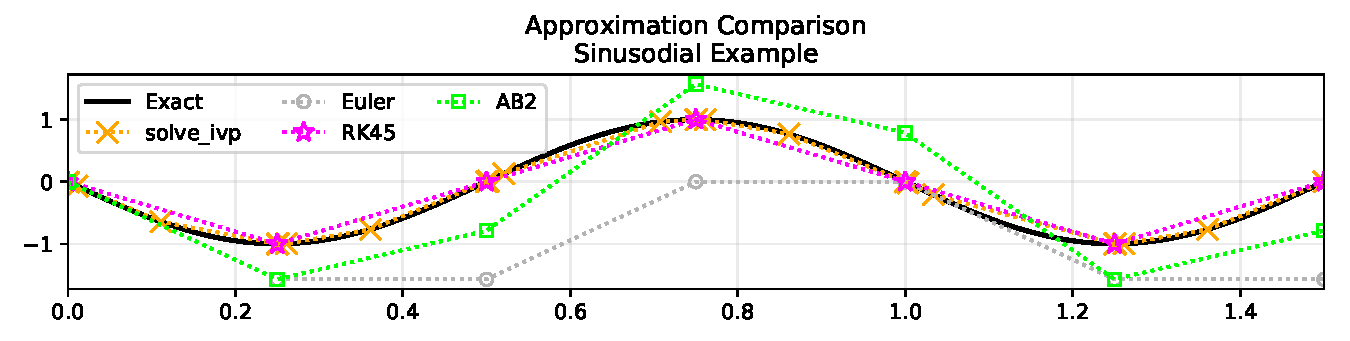
\includegraphics[width=\linewidth]{figures/sinEx}
	\caption{Approximation comparison of a sinusoidal function.}
	\label{fig: sin ex}
\end{figure}

\begin{figure}[H]
	\centering
	\footnotesize
	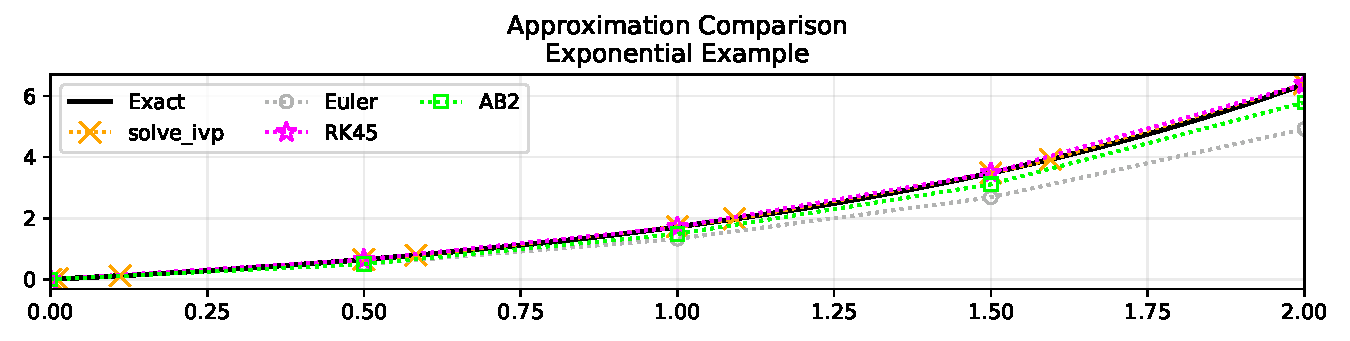
\includegraphics[width=\linewidth]{figures/expEx}
	\caption{Approximation comparison of an exponential function.}
	\label{fig: exp ex}
\end{figure}


\begin{figure}[H]
	\centering
	\footnotesize
	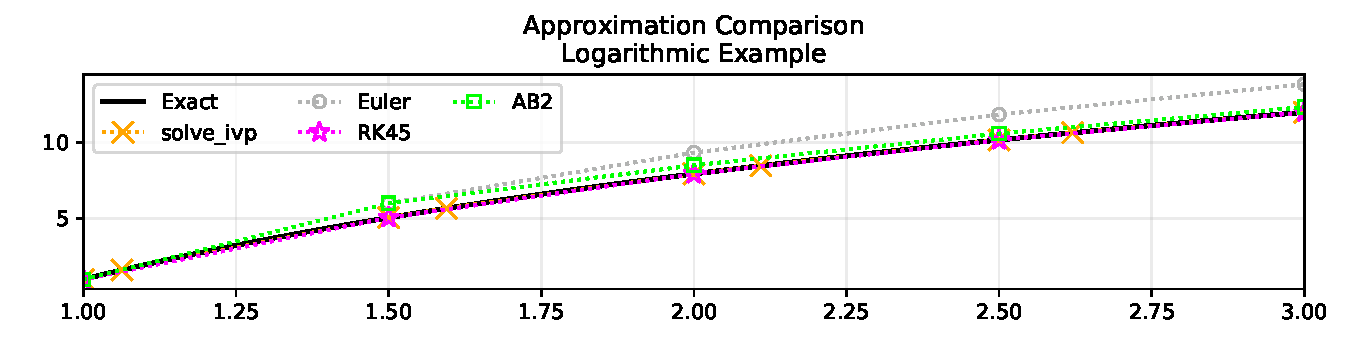
\includegraphics[width=\linewidth]{figures/logEx}
	\caption{Approximation comparison of a logarithmic function.}
	\label{fig: log ex}
\end{figure}







% used to solve state space equations used in governor dynamics
\paragraph{sig.lsim}
To process a signal through a Laplace block, the block is first transformed into state space matrices and then inserted into sig.lsim for a linear simulation.
This is used in all dynamic processes of PSLTDSim including governor states, filter and delay blocks.

% process to transform simple laplace blocks to state space

\end{document}